\documentclass{article}
\usepackage[utf8]{inputenc}
\usepackage{pl_paper}

\title{Concurrent Programming Languages}
\author{
    Nick LaPosta & Chris Heisler & Derek Gaffney \email lapost48@students.rowan.edu & heislerc0@students.rowan.edu  & gaffneyd4@students.rowan.edu \and John Bucknam & Johnathon Saunders & Jatin Bhakta \email bucknamj8@students.rowan.edu & saundersj0@students.rowan.edu & bhaktaj7@students.rowan.edu
    }
\date{February 21, 2017}

\begin{document}

\maketitlepage

\tableofcontents

\begin{multicols*}{2}\raggedcolumns\pagenumbering{arabic}

    \section{Introduction}

        There has recently been a shift in the focus of computer hardware manufacturers. Most manufacturers spent their research and development on increasing the clock speed of their hardware to make computation faster. However, lately has been a plateau on clock speed resulting in a new way to increase processing speed. The way many manufacturers are increasing the computational power of computers is by adding multiple computational cores on a  single chip. This allows programs to run multiple computations at the same time which can cut the runtime of processes drastically. Multiple cores have been common on larger hardware, such as GPUs, but there hasn't been much focus on truly expanding the number of cores on a CPU. However, with multiple cores becoming more common programmers will need to be able to make use of them effectively if they want to gain any benefit. Admittedly, there are some applications that multiple cores can't increase performance; however, many applications can be easily converted to run parallel on multiple cores.

Although many applications can be easily be converted to run parallel, some languages make that task less trivial than it should be. The design of new languages that are intended to be used for parallel computation is vital to the advancement of computation. Some languages try to build libraries into the language to handle this multiple core processing, such as Java, but they are hard to work with. In this paper we are going to discuss concurrent programming languages and what affect they have on basic and advance programs. We will be focusing on Go (a language created by Google and used for servers), Swift (a programming language that focuses on increasing time performance of other applications for scientific programming), and Clojure (a dynamic, Lisp dialect with a focus on concurrency).

\subsection{Programming Problem}
    The problem we will be solving is a simple two matrix multiplication. The reason we chose this problem is because it is an operation that is typically handled by an external library, such as NumPy \cite{numpy}, but can easily be parallelized as it is many discrete operations that are independent of one another. We will be multiplying square matrices of the following sizes: 100, 250, 500, 750, 1000, 1500, 2000. With this we will be able to show how performance changes with increased data size. We will compare the languages mentioned earlier to the Thread implementation of Java. Since Java is not optimized to be a parallel programming language we are expecting each of the optimized languages to exceed its performance.

\subsection{Concurrency Limit \& Bandwidth}
    The limit of concurrency is dependent on not only how much you can work on your problem separately, but also a limitation on hardware and bandwidth. Our given programming problem is an easy problem to apply concurrently, but we can't run 200 threads with only 8 cores, and as we parallelize our threads, we will find a lower utilization in general for a single thread that could lead to a longer execution time. This bottlenecking is a common issue in concurrency, but is one of several. Although concurrency is incredibly important for performance, large amounts can lead to issues with memory bandwidth and cache\cite{cuppu2001concurrency}, which can cause bottle-necking. This could be a limitation for our matricies as well, leading to negative results with incredibly large matrix multiplication.


    \section{Go}

        \goColor
\subsection{Introduction to the Go Programing Language}
	The Go programming language was designed by Robert Griesemer, Rob Pike and Ken Thompson. A portion of their design focused on creating a new language with support for networked and multi-core computing. Go’s concurrency implementation builds upon ideas from past languages, such as Newsqueak, Alef and Limbo, and C.A.R. Hoare’s 1978 paper, Communicating Sequential Processes (CSP), a formal language for writing concurrent programs. \cite{prell:hal-00718924} This implementation differs from the usual methodology of locks and threads.
	The core principle of Go is to reduce complexities present in modern programming languages and concurrent programming is one such complexity. The new language provides an approach in which shared values are easily passed between sequential processes. The medium of communication, variable passing, is referred to as a channel. CSP introduced the concept of channels for interprocess communication in a book written by Hoare, published after his original paper. This method of operation, in which processes (goroutines) communicate through channels, is analogous to the programming style of message passing. The use of channels ensures that variables are never actively chard by separate processes, thus data races can never occur. The Go concurrent methodology can be reduced to its slogan, “Do not communicate by sharing memory; instead, share memory by communicating”. \cite{website:go-lang-documentation}
	Go’s concurrent programming is based on two fundamentals, goroutines and channels. Goroutines have a simple model and can be thought as lightweight threads. Channels serve to handle both communication and synchronization. By default Go’s channels are synchronous, and channels are unbuffered when a buffer size is not specified. \cite{prell:hal-00718924} The specifics of Go’s channel will be discussed later, but first we will cover goroutines, for channels exist to serve them. Lastly, we will discuss parallelization in Go and apply it within our matrix multiplication code.
\subsection{Goroutines}
	The term goroutine was made because existing terms for concurrent processes, such as threads, coroutines, process, etc., convey a meaning that inaccurately describes how Go executes functions concurrently. The goroutine model is simple and lightweight, hiding man of the complexities of thread creation and management. Goroutines execute in the same address space, and memory allocation starts at the cost of a small stack space and grows by allocating and freeing as heap storage requires. Goroutines are multiplexed onto OS threads, not process threads, therefore in one goroutine is to block the others will continue to execute.\cite{website:go-lang-documentation}
	A goroutine is created simply by prefixing the keyword \emph{go} to a function call.
\begin{lstlisting}[language=Go]
go innerprod(a, b, ch)
// Execute the inner product function
// concurrently as a goroutine,
// do not wait for it to finish.
\end{lstlisting}
Function innerprod(a, b, ch) takes the inner product of a row vector \emph{a} and column vector \emph{b}. The parameter \emph{ch} is of type channel, which will be discussed thoroughly in the next section. Then, a detailed explination of the function will provided in our matrix multiplication program section. To digress, the important point here is to convey the simplicity of creating a goroutine, that any function may be run concurrently by prefixing the keyword \emph{go}. However, if the function does not recieve a channel, then the goroutine will not be able to properly return variables or signal its completion.
\begin{lstlisting}[language=Go]
func badgoroutine(a, b){
	result := go innerprod(a, b)
	fmt.Println(result)
}
\end{lstlisting}
A goroutine should never be used as shown above. In fact this code has created a race condition, and is general example of bad concurrent programming.
	One last feature to note, Go function lterals are closures, thus ensureing variables referred to by the function remain until they are no longer needed. A code snippet from the Golang documentation demostrates the use of a function literal in a goroutine function literal.
\begin{lstlisting}[language=Go]
func Announce(message string,
	delay time.Duration) {

    go func() {
        time.Sleep(delay)
        fmt.Println(message)
    }()
    /* Note the parentheses - must
       call the function. */
}.
\end{lstlisting}
\subsection{Channels}
Channels use the make function to allocate themselves, the resulting value references the underlying data structure. If you add an integer value as a second parameter (you do not have to add an integer as the second parameter because it is optional) it sets the buffer size of that channel. For example (all following examples were obtained from \cite{website:go-lang-documentation}):
\begin{lstlisting}[language=Go]
ci := make(chan int)
\end{lstlisting}
Creates a channel on integers that is unbuffered. Interestingly because the second parameter is optional if not entered its default is 0 so it is the same as coding:
\begin{lstlisting}[language=Go]
cj := make(chan int, 0)
\end{lstlisting}
But if you do enter something other than 0 like follows:
\begin{lstlisting}[language=Go]
cs := make(chan int, 100)
\end{lstlisting}
It creates a buffered channel of pointers to integers.
If a channel is unbuffered Go will use a combination of communication and synchronization to ensure that the goroutines are within a known state.  A use full demonstration of using channels with goroutines is to having a channel on a variable do a sort within goroutine. Then give a value to that while everything outside the routine continues until it arrives at the channeled variable. This would cause it to wait until the goroutine operating on the variable has finished before continuing.  This is a general implementation of what I have just described:
\begin{lstlisting}[language=Go]
c := make(chan int)
/* makes an unbuffered
   channel of type int.
   Start a goroutine wait for
   it to complete then signal
   on the channel. */
go func() {
    list.Sort()// sorts some list
    c <- 1
    /* Send a signal,
       the value does not matter
       or this demonstration. */
}()
doSomethingForAWhile()
<-c   // Waits for sort to finish;
\end{lstlisting}
The blockers, in this case c, will block until data is received. If the channel is an unbuffered channel the sender will block until it receives a value. Otherwise if the channel is buffered the sender only blocks as until the buffer has been filled. This mean that if a buffer is full it will wait until a receiver tries to retrieve it.
	A buffered channel can be used as a type of semaphore. For instance this example limits throughput:
\begin{lstlisting}[language=Go]
func handle(queue chan *Request) {
    for r := range queue {
        process(r)
    }
}

func Serve(clientRequests chan
	*Request, quit chan bool) {

    // Start handlers
    for i := 0; i < MaxOutstanding;
    i++ {
        go handle(clientRequests)
    }
    <-quit
   // Wait to be told to exit.
}
\end{lstlisting}
A very important property to remember in go is the first class values can be passed around like any other values. This can be used to to create safe and parallel demultiplexing. As an example we will be dissecting the handle function from above. If you recall, in the previous example, we did not define the type it was handling. If they type has a channel where it can reply the client is able to determine it own path to the answer. This is a schematic of type Result :
\begin{lstlisting}[language=Go]
type Request struct {
    args        []int
    f           func([]int) int
    resultChan  chan int
}
\end{lstlisting}
The client gives a function, argument, and channel inside a request object to receive the answer.
\begin{lstlisting}[language=Go]
func sum(a []int) (s int) {
    for _, v := range a {
        s += v
    }
    return
}

request := &Request{[]int{3, 4, 5},
	 	sum, make(chan int)}
// Send request
clientRequests <- request
// Wait for response.
fmt.Printf("answer: %d\n",
		<-request.resultChan)
\end{lstlisting}
On the back end the handler is the only thing that changes.
\begin{lstlisting}[language=Go]
func handle(queue chan *Request) {
    for req := range queue {
        req.resultChan <- req.f(
			    req.args)
    }
}
\end{lstlisting}
This is the general framework for a rate-limited, parallel, non-blocking RPC system.
\subsection{Parallelization}
“Another application of these ideas is to parallelize a calculation across multiple CPU cores. If the calculation can be broken into separate pieces that can execute independently, it can be parallelized, with a channel to signal when each piece completes.”\cite{website:go-lang-documentation}
\emph{Parrallelization is to be discussed in more details.}
\subsection{Concurrent Matrix Multiplication Results}
\emph{Code and results to be added later.}


    \section{Swift-Lang}

        \swiftColor
When dealing with large collections of data or several different programs, it can be troublesome to configure individual settings or to have a single script run through. Doing this on a normal programming language would require more effort, and may have trouble dealing with either larger amounts of data or is unable to speed up individual tasks. This becomes more pertinent as we use parallel computing to hasten our programs, but how do we manage several programs with larger datasets?

Swift is an implicit, "parallel", scripting language that heavily aids with these distributed tasks, allowing for several of the same or different programs to run concurrently. Although it is currently not a full version, Swift has been used for several scientific programs such as protein structure prediction, glass structure modeling, and modeling climate and economics. There has also been discussion for petascale supercomputing using Swift as the parallel computing language \cite{wilde2009parallel}

What makes Swift so powerful is its built-in support for bash, allowing different Swift applications to run bash commands. This feature allows it to run many different programs in several different programming languages, as they use bash to process them. But how does Swift perform these tasks?

\subsection{Language Basics}
    Swift is very similar in syntax to languages such as C and Java, but they don't have any object type or class type. Instead, they use data structures, references, and some atomic structures to define their data as well as how they use them for different Swift procedures, instructions, and external calls. \cite{website:swift-lang-documentation}

    \subsubsection{Types}
        Swift is strongly-typed, with types being \textit{atomic} or \textit{composite}. An atomic type can be a \textit{primitive} (\texttt{int}, \texttt{string}, \texttt{float}, or \texttt{boolean}) or a \textbf{marker} type, which signifies that data for that variable is stored in a single file. As for composite types, they can either be arrays (integers or another primitive type for associative arrays) and a structure used to contain other variables.

        \begin{lstlisting}[language=swift]
// ----------------
// Atomic Types
// ----------------

// Primitives
string name = "Nick LaPosta";

// Marker Type
type image;
image photo <"lena.png">;

// ----------------
// Composite Types
// ----------------

// Arrays
string coolPeople[] = ["John Bucknam"];
float[string] constants;
constants["pi"] = 3.1415926535;

// Structures
type circle {
    int radius;
    string color;
};
        \end{lstlisting}

    \subsubsection{Procedures}
        Similar to method and functions in other languages, Swift create \textit{procedures} that can be called in the script after declaration. There are primariliy two types of procedures, compound procedures and atomic procedures.

        Compound procedures run solely Swift operations and other procedures, and can have several inputs and outputs.

        \begin{lstlisting}[language=swift]
(int output) addtwo (int input) {
    output = input + 2;
}

int test = 2;
int y;

y = addtwo(test);
        \end{lstlisting}

        Atomic procedures run external, executable program such as bash commands, as well as handles the mapping to different command line arguments. They differ from compound procedures with an \texttt{app} keyword in the beginning of the procedure

        \begin{lstlisting}[language=swift]
app sayHello (string name) {
    echo "Hello world, I am " name;
}

sayHello("Nick");
    \end{lstlisting}

    \subsubsection{Operators}

    +, -, *, /, etc.

\subsection{Runtime Environment}

How it performs reliable executions on external programs, as well as avoiding job submission penalties. \cite{wilde2011swift}

\subsection{Applications}

What has it been commonly used for? This consists of several, difficult problems in the scientific community and how they rely on parallelization when using large clusters or supercomputers. \cite{wilde2009parallel} \cite{hategan2011coasters}

\subsection{Performance}

How well does it utilize CPUs or perform specific jobs? \cite{wilde2011swift}


    \section{Clojure}

        \clojureColor
\subsection{Code Test}

    \begin{lstlisting}[language=clojure]
(ns helloworld.core)

(defn -main []
    "I can say 'Hello World'."
    (println "Hello, World!"))
    \end{lstlisting}


    \section{Conclusion}

        From these three languages we can see the importance of parallelization and concurrency in different applications, as well as how greatly each vary. This can be from specific inspiration or reasoning to solve a problem, as Go and Clojure have a range of tools and larger forms of importing than Swift, which focuses on the implementations of other languages and applications.

Each also have their own way of dealing with lack of hardware or dealing with concurrency to the point where variable initialization is taken into account as to what default values will be read if nothing reaches to assign it. It has also been asked if the variable should be assigned before reading as well, creating interesting paradigms and designs for each language.

Their applications have wide variations, from scientific computing in clusters or grids to working with servers or local applications. This expanse in usage and features is what makes these languages not only verbose, but also fast, using concurrency to speed up their general performance.

\subsection{Comparison: Java vs. Go vs. Clojure}
    Earlier we described a programming problem that we gave each of our programs to solve, and later described how Swift isn't meant for this type of use and focuses more on optimizing different applications, leaving us Go and Clojure. We will be comparing these two with Java, using several different matrix sizes (NxN) as the input and seeing how it corresponds with its execution speed.

    In our Clojure and Go sections, we saw how the execution time output for each matrix size NxN. For our Java implementation using threads, we received our own set of results.
    \\~\\
    \begin{tabular}{ | l | l | l | p{5cm} |}
    \hline
    N & Average Number of Seconds to Completion \\ \hline
    100 & 0.08 \\ \hline
    250 & 0.28 \\ \hline
    500 & 11.3 \\ \hline
    750 & 25.5 \\ \hline
    1000 & 45.1 \\ \hline
    1500 & 101.6 \\ \hline
    2000 & 181.3 \\ \hline

    \hline
    \end{tabular}\\~\\

    Using our previous results as well as our Java results, we created a graph comparing each language implementation on the number of seconds need to complete the matrix multiplication to the size of the square matrix used. We found that Java, as expected, performed the worse in general while Clojure beat our Go implementation when using larger matricies.

    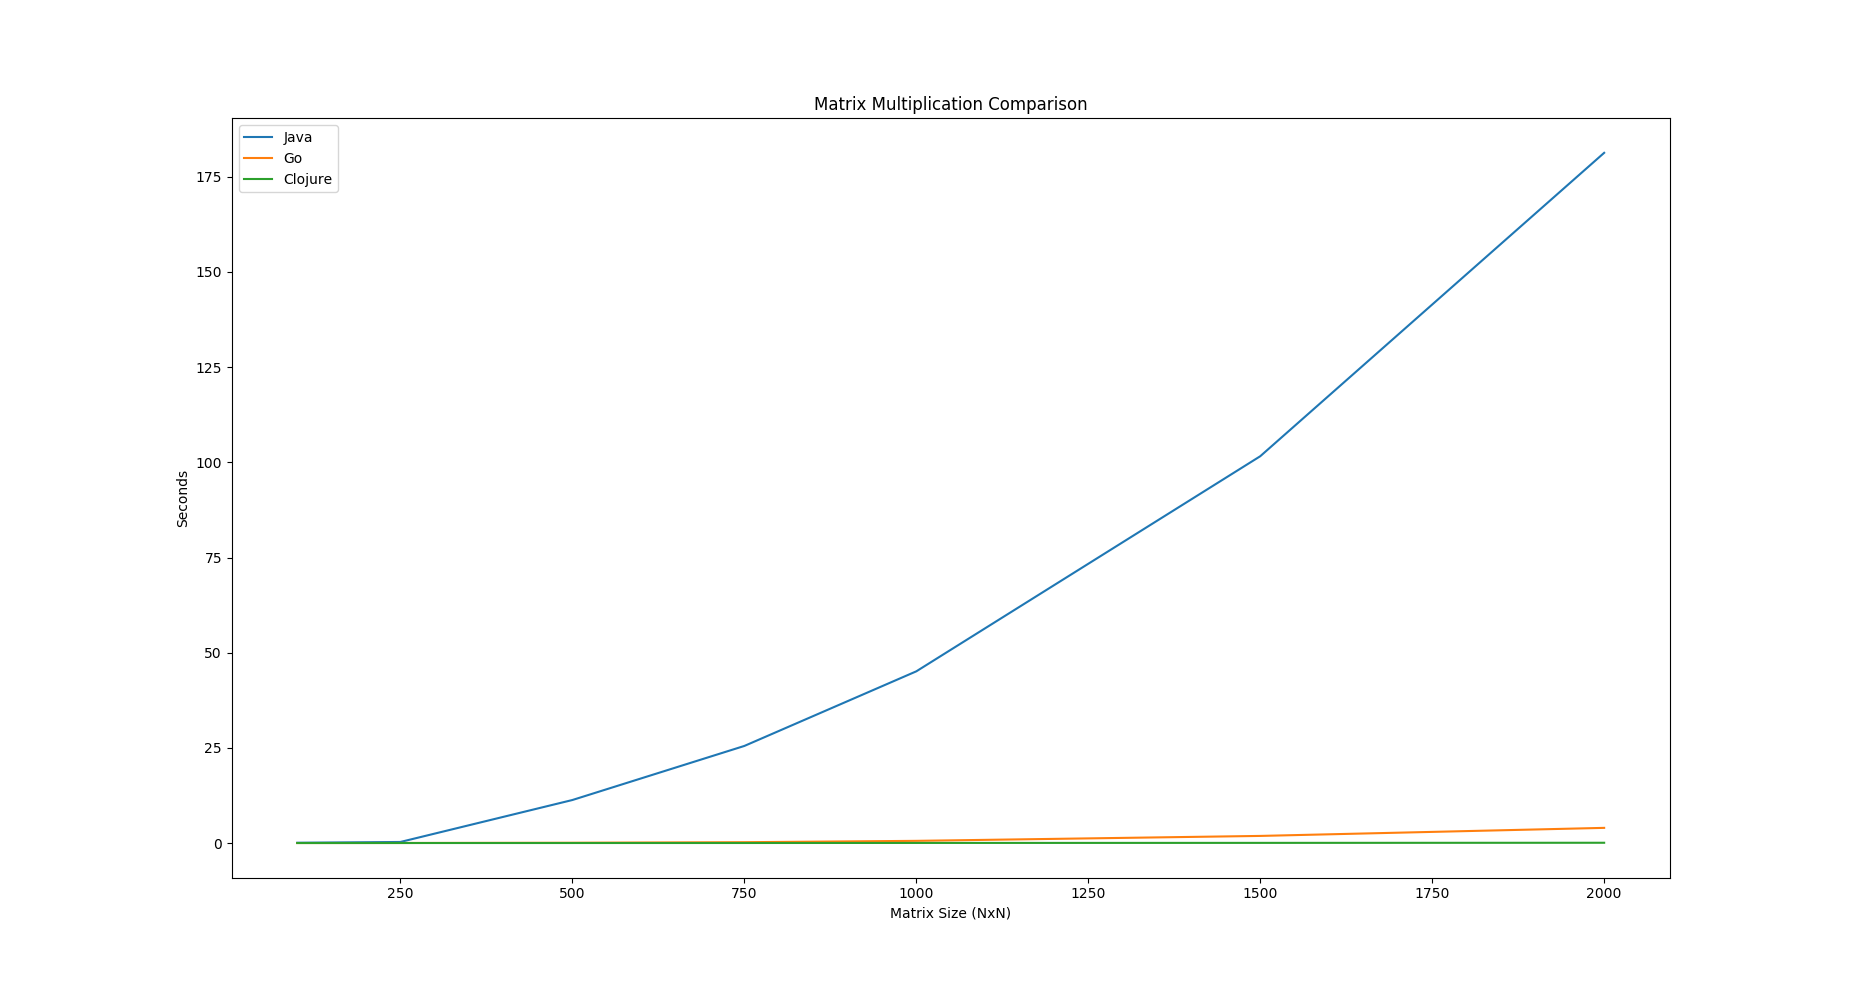
\includegraphics[width=\linewidth,keepaspectratio]{conclusion/comparison.png}

    We would like to do larger comparisons with more hardware, as our brief test could have depending on what hardware each of us used in our implementation and how well they can implement other forms of software such as CUDA or larger frameworks. However, this test does show the improvements when implementing a concurrent language compared to a non-concurrent language, even comparing two languages using the JVM (Java and Clojure).


\end{multicols*}

\startofappendix
\goColor
\begin{appendix}{Go}
    \addcodeappendix{Go}{matmul/go/matrixmult.go}
    \addcodeappendix{Go}{matmul/go/matrix/matrix.go}
\end{appendix}
\swiftColor
\begin{appendix}{Java}
    \addcodeappendix{Java}{matmul/java/Driver_1.java}
    \addcodeappendix{Java}{matmul/java/Driver_2.java}
\end{appendix}
\clojureColor
\begin{appendix}{Clojure}
    \addcodeappendix{Clojure}{matmul/clojure/matrixmult_1.cjl}
    \addcodeappendix{Clojure}{matmul/clojure/matrixmult_2.cjl}
\end{appendix}

\addtocontents{toc}{\protect\newpage}
\bibliography{references}{\pagenumbering{gobble}}
\bibliographystyle{acm}

\end{document}
